\section{Wave Physics Model }

The sea surface height $\eta(x, z, t)$ is modeled as a superposition of multiple sinusoidal components, mimicking a simplified Gerstner Wave and following Pierson-Moskowitz spectrum. The total displacement at any point $\mathbf{p}$ is the sum of $n$ wave harmonics:

\begin{equation}
\eta(\mathbf{p}, t) = \sum_{i=1}^{n} A_i \cdot \sin(\mathbf{k}_i \cdot \mathbf{p}_x + \omega_i t) \cdot \cos(\mathbf{k}_{i,z} \cdot \mathbf{p}_z \cdot \phi + \omega_i t)
\end{equation}


Where: $A_i$ is the amplitude of the $i$-th harmonic. $\mathbf{k}_i$ is the wave vector (determining frequency and direction). $\omega_i$ is the angular frequency (phase speed). $\phi$ is a directional interference constant (set to $0.8$ in this model to avoid perfect symmetry).The implementation categorizes these into three distinct scales:
Primary Swells: Low frequency, high amplitude (e.g., $f=0.02, A=0.8$).
Turbulent Mid-levels: Moderate frequency for sea-state texture.
Capillary Ripples: High frequency, low amplitude for surface detail.
Values used in simulation are visible in table \ref{tab:wave_parameters}.



\begin{figure}[htbp]
    \centering
    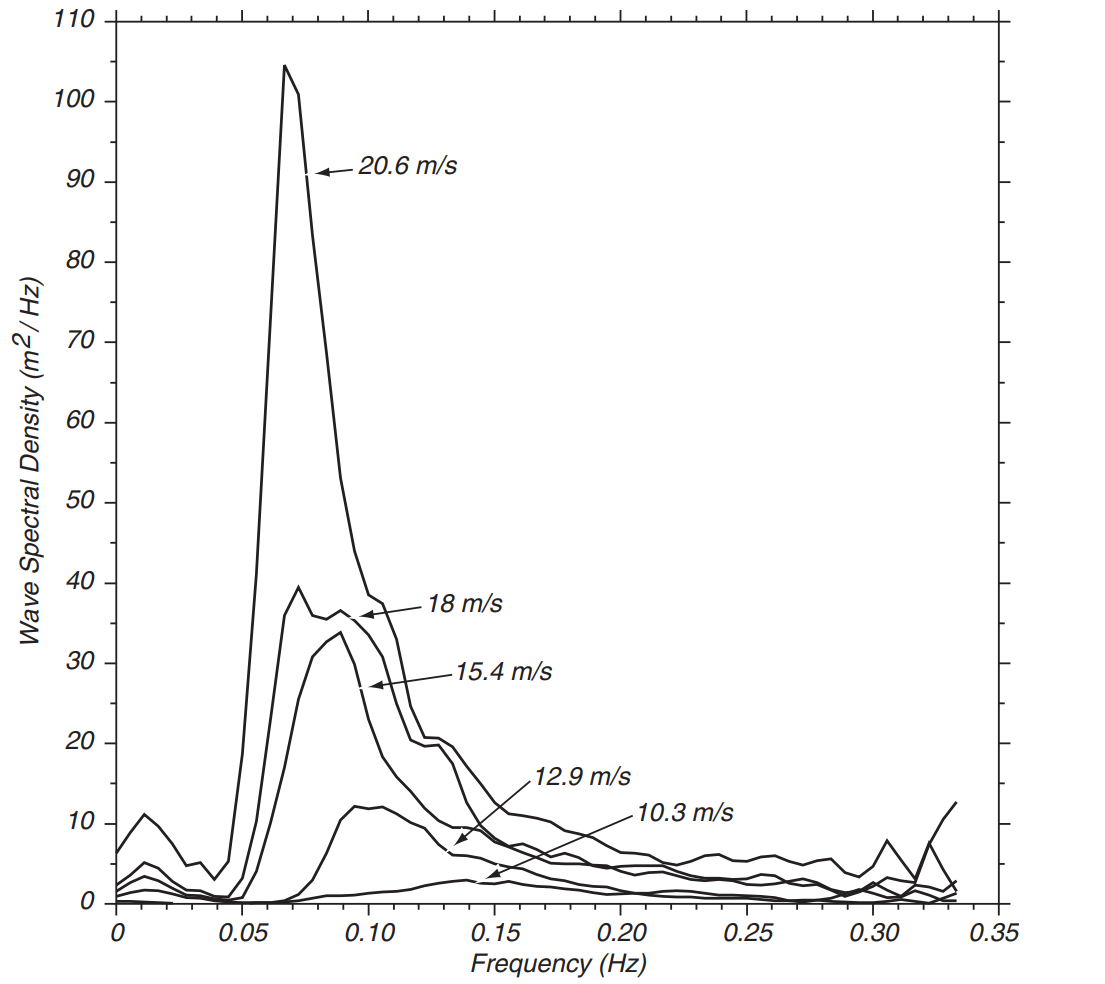
\includegraphics[width=0.7\textwidth]{images/MoskowitzSpectra.png}
    \caption{Wave spectra for different wind speeds according to Moskowitz (1964). \cite{alves2003revisiting}}
    \label{fig:moskowitz_spectra}
\end{figure}


\begin{table}[h]
\centering

\caption{Spectral Parameters for Procedural Wave Synthesis}
\label{tab:wave_parameters}
\begin{tabular}{lccc}
\toprule
\textbf{Wave Category} & \textbf{Frequency} ($f$) & \textbf{Speed} ($v$) & \textbf{Amplitude} ($A$) \\ 
\midrule
Primary Swell 1        & 0.02 Hz                 & 1.2 m/s             & 0.80 m                          \\
Primary Swell 2        & 0.04 Hz                 & 1.5 m/s             & 0.50 m                          \\
Mid-level Turbulence   & 0.10 Hz                 & 2.2 m/s             & 0.20 m                          \\
Secondary Turbulence   & 0.18 Hz                 & 1.8 m/s             & 0.15 m                          \\
Surface Micro-Ripple   & 0.45 Hz                 & 3.0 m/s             & 0.05 m                          \\
Capillary Ripple       & 0.80 Hz                 & 4.2 m/s             & 0.02 m                          \\ \bottomrule
\end{tabular}
\end{table}



To calculate buoyancy forces, the surface normal $\mathbf{\hat{n}}$ must be derived. Rather than analytical differentiation, which becomes computationally expensive as $n$ increases, a Finite Difference Method is used. By sampling the height at four orthogonal offsets around a point $\mathbf{p}$, the slope is determined:

\begin{align}
\frac{\partial \eta}{\partial x} \approx \frac{\eta(x-\epsilon, z) - \eta(x+\epsilon, z)}{2\epsilon}\\
\frac{\partial \eta}{\partial z} \approx \frac{\eta(x, z-\epsilon) - \eta(x, z+\epsilon)}{2\epsilon}
\end{align}


The resulting normal vector is:

\begin{equation}
\mathbf{\hat{n}} = \text{normalize}\left( \frac{\partial \eta}{\partial x}, 1.0, \frac{\partial \eta}{\partial z} \right)
\end{equation}

This is later used in Physics Model to calculate Wave-Slope Dynamics.


\begin{figure}[htbp]
    \centering
    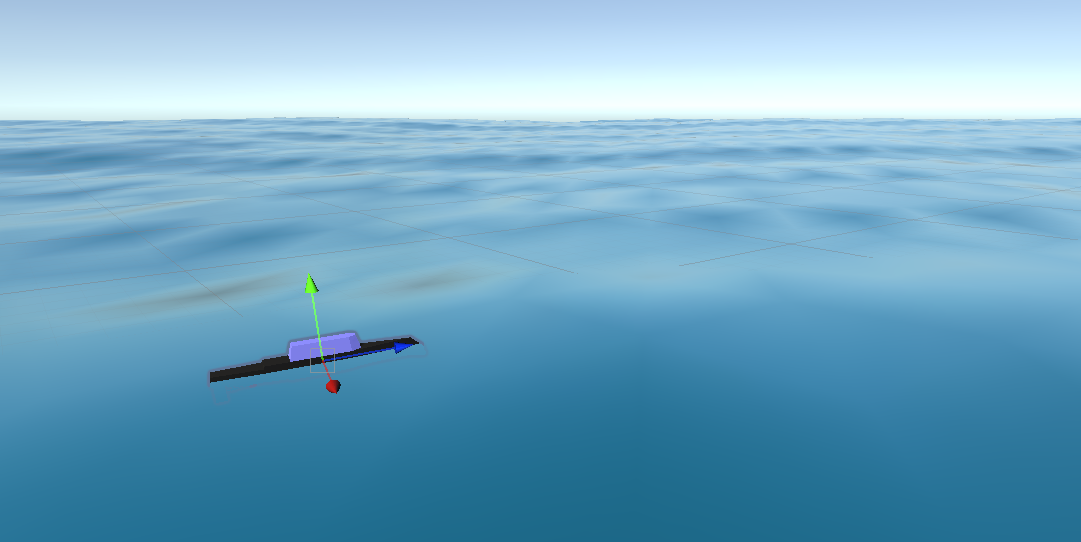
\includegraphics[width=0.8\textwidth]{images/waves_system2.png}
    \caption{Waves simulation resoults.}
    \label{fig:waves_model}
\end{figure}